\documentclass[landscape]{article}
\usepackage[margin=1in]{geometry}
\usepackage{clrscode3e}
\usepackage{amsmath}
\usepackage{graphicx}

\newcommand{\bi}{\begin{itemize}}
\newcommand{\ii}{\item}
\newcommand{\ei}{\end{itemize}}
\newcommand{\bn}{\begin{enumerate}}
\newcommand{\en}{\end{enumerate}}
\newcommand{\set}[1]{\ensuremath{\left\{#1\right\}}}
\newcommand{\pr}[1]{\ensuremath{\mbox{Pr}\left\{#1\right\}}}
\newcommand{\flr}[1]{\ensuremath{\left\lfloor#1\right\rfloor}}
\newcommand{\ceil}[1]{\ensuremath{\left\lceil#1\right\rceil}}

\newcommand{\sect}[1]{\newpage{\bf #1}}

\setlength{\parindent}{0in}

\title{Notes on Heapsort}
\author{Geoffrey Matthews}
\begin{document}
\maketitle
\titlepage
\huge

\sect{Heapsort}
\bi
\ii $O(n\lg n)$ worst case --- like merge sort
\ii Sorts in place --- like insertion sort
\ii Combines best of both algorithms
\ei

\sect{Heaps}
\bi
\ii A nearly complete binary tree.
\ii {\bf Height:} number of edges on longest path from node to leaf
\ii Stored as an array $A$
\bi
\ii Root at $A[1]$
\ii Left child at $A[2i]$
\ii Right child at $A[2i+1]$
\ii Parent of $A[i]$ at $A[\lfloor i/2\rfloor]$
\ei
\ii Computing very fast
\ei
  
\sect{Example Max-heap}

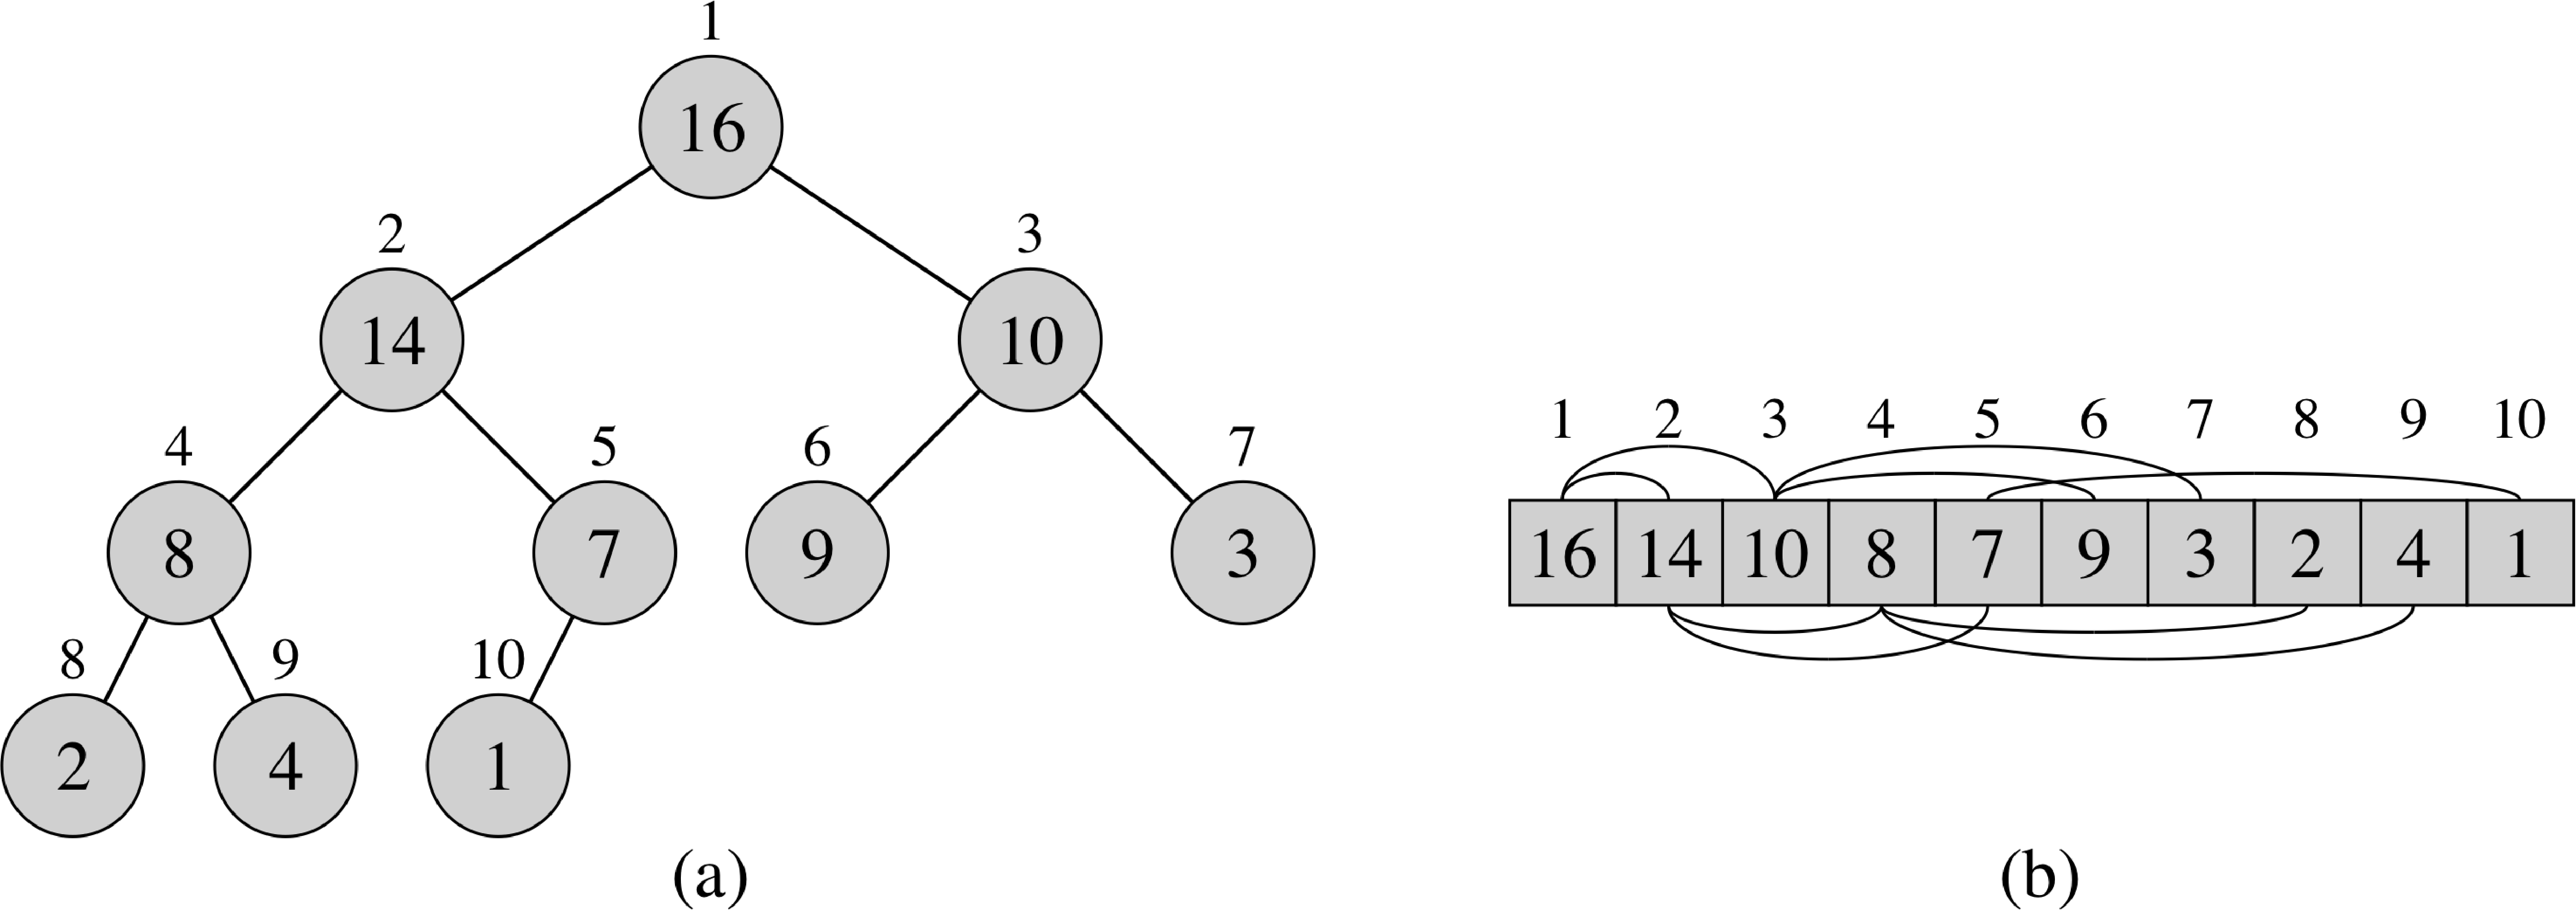
\includegraphics[width=\textwidth]{Fig-6-1.pdf}

\bi
\ii For max-heaps: $A[\mbox{\sc Parent}(i)] \geq A[i]$
\ii Induction can prove largest element is at root.
\ei


\sect{\sc Max-Heapify}
\bi
\ii Preconditions:
\bi
\ii $A[i]$ may be smaller than its children.
\ii Left and right subtrees of $i$ are max-heaps.
\ei
\ii Postcondition: subtree rooted at $i$ is a max-heap.
\ei
\hrulefill
\begin{codebox}
  \Procname{$\proc{Max-Heapify}(A,i,n)$}
  \li $l \gets \proc{Left}(i)$
  \li $r \gets \proc{Right}(i)$
  \li \If $l \leq n$ and $A[l] > A[i]$ \Do
  \li $largest \gets l$
  \End
  \li \Else $largest \gets i$
  \li \If $r\leq n$ and $A[r] > A[largest]$ \Do
  \li ${largest} \gets r$ \End
  \li \If ${largest} \not = i$ \Do
  \li exchange $A[i]$ with $A[largest]$
  \li $\proc{Max-Heapify}(A,largest,n)$
\End
\end{codebox}


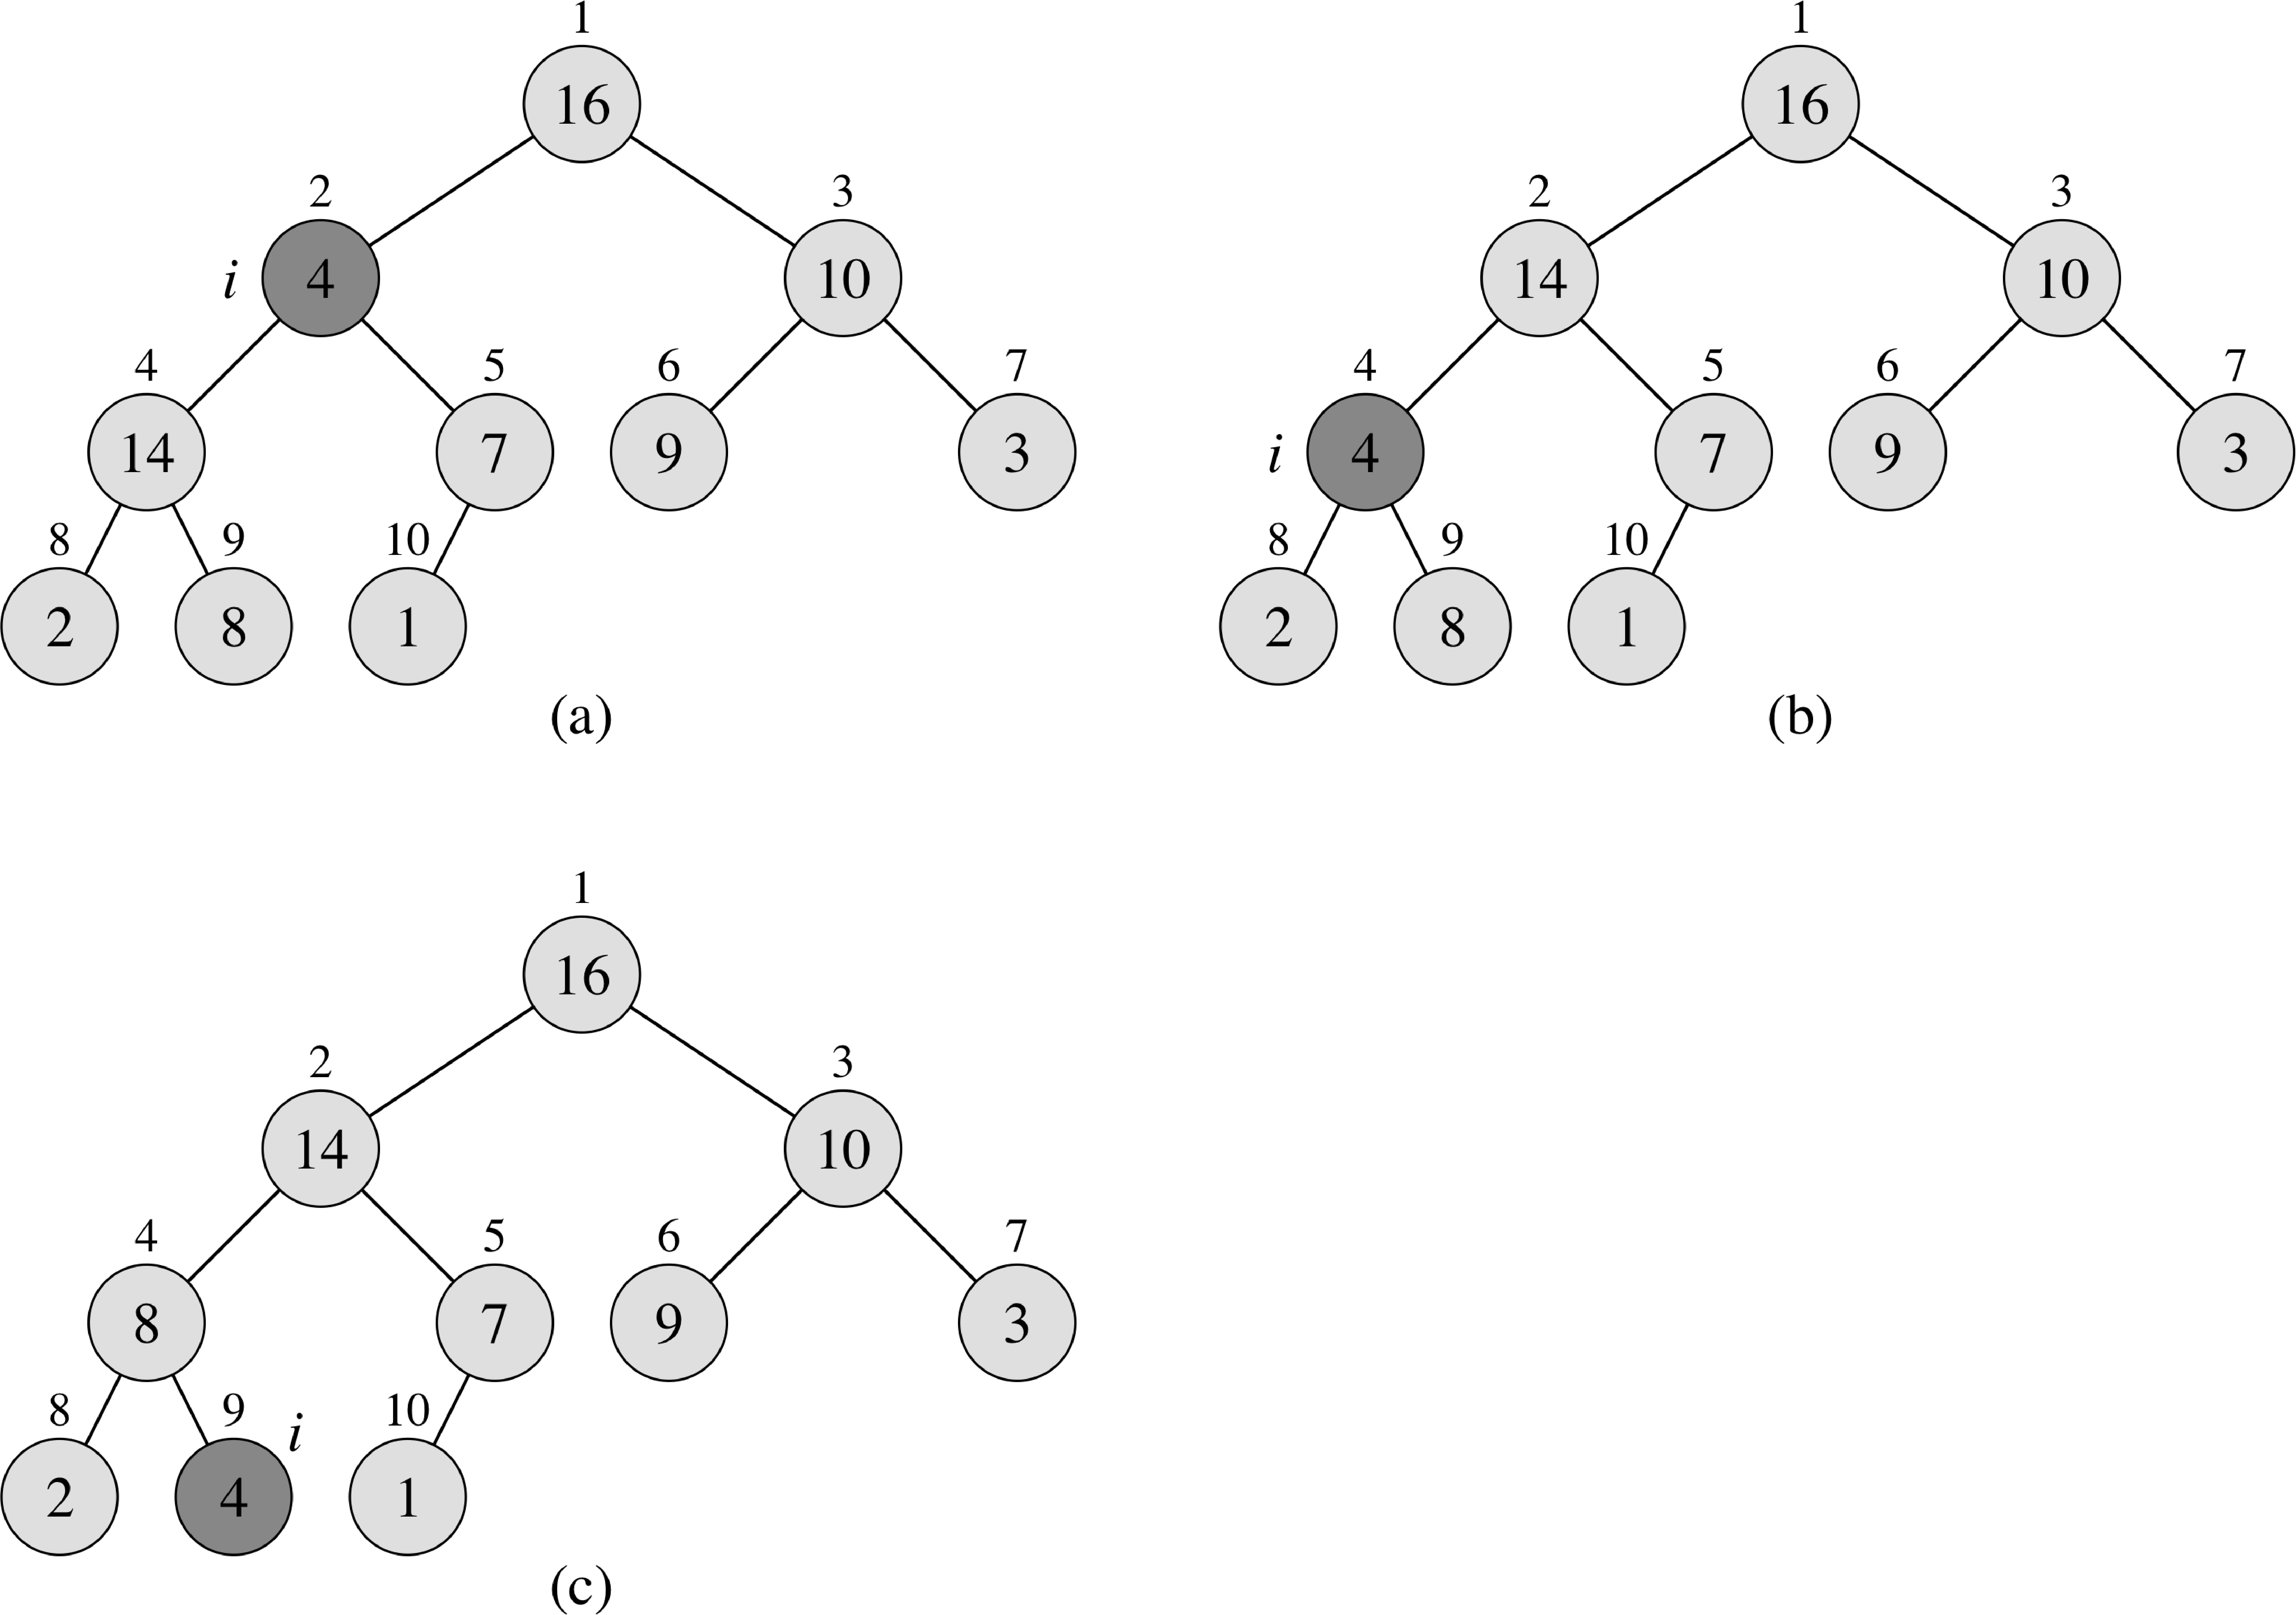
\includegraphics[width=\textwidth]{Fig-6-2.pdf}

\sect{Time for {\tt Max-Heapify}}
\bi
\ii
$O(\lg n)$
\ii
Why?
\ei

\sect{\sc Build-Max-Heap}
\bi
\ii If $A$ is not a max-heap, this will make it one.
\ei
\begin{codebox}
  \Procname{$\proc{Build-Max-Heap}(A,n)$}
  \li \For $i=\lfloor{n/2}\rfloor \Downto 1$ \Do
  \li $\proc{Max-Heapify}(A,i,n)$
  \End
\end{codebox}

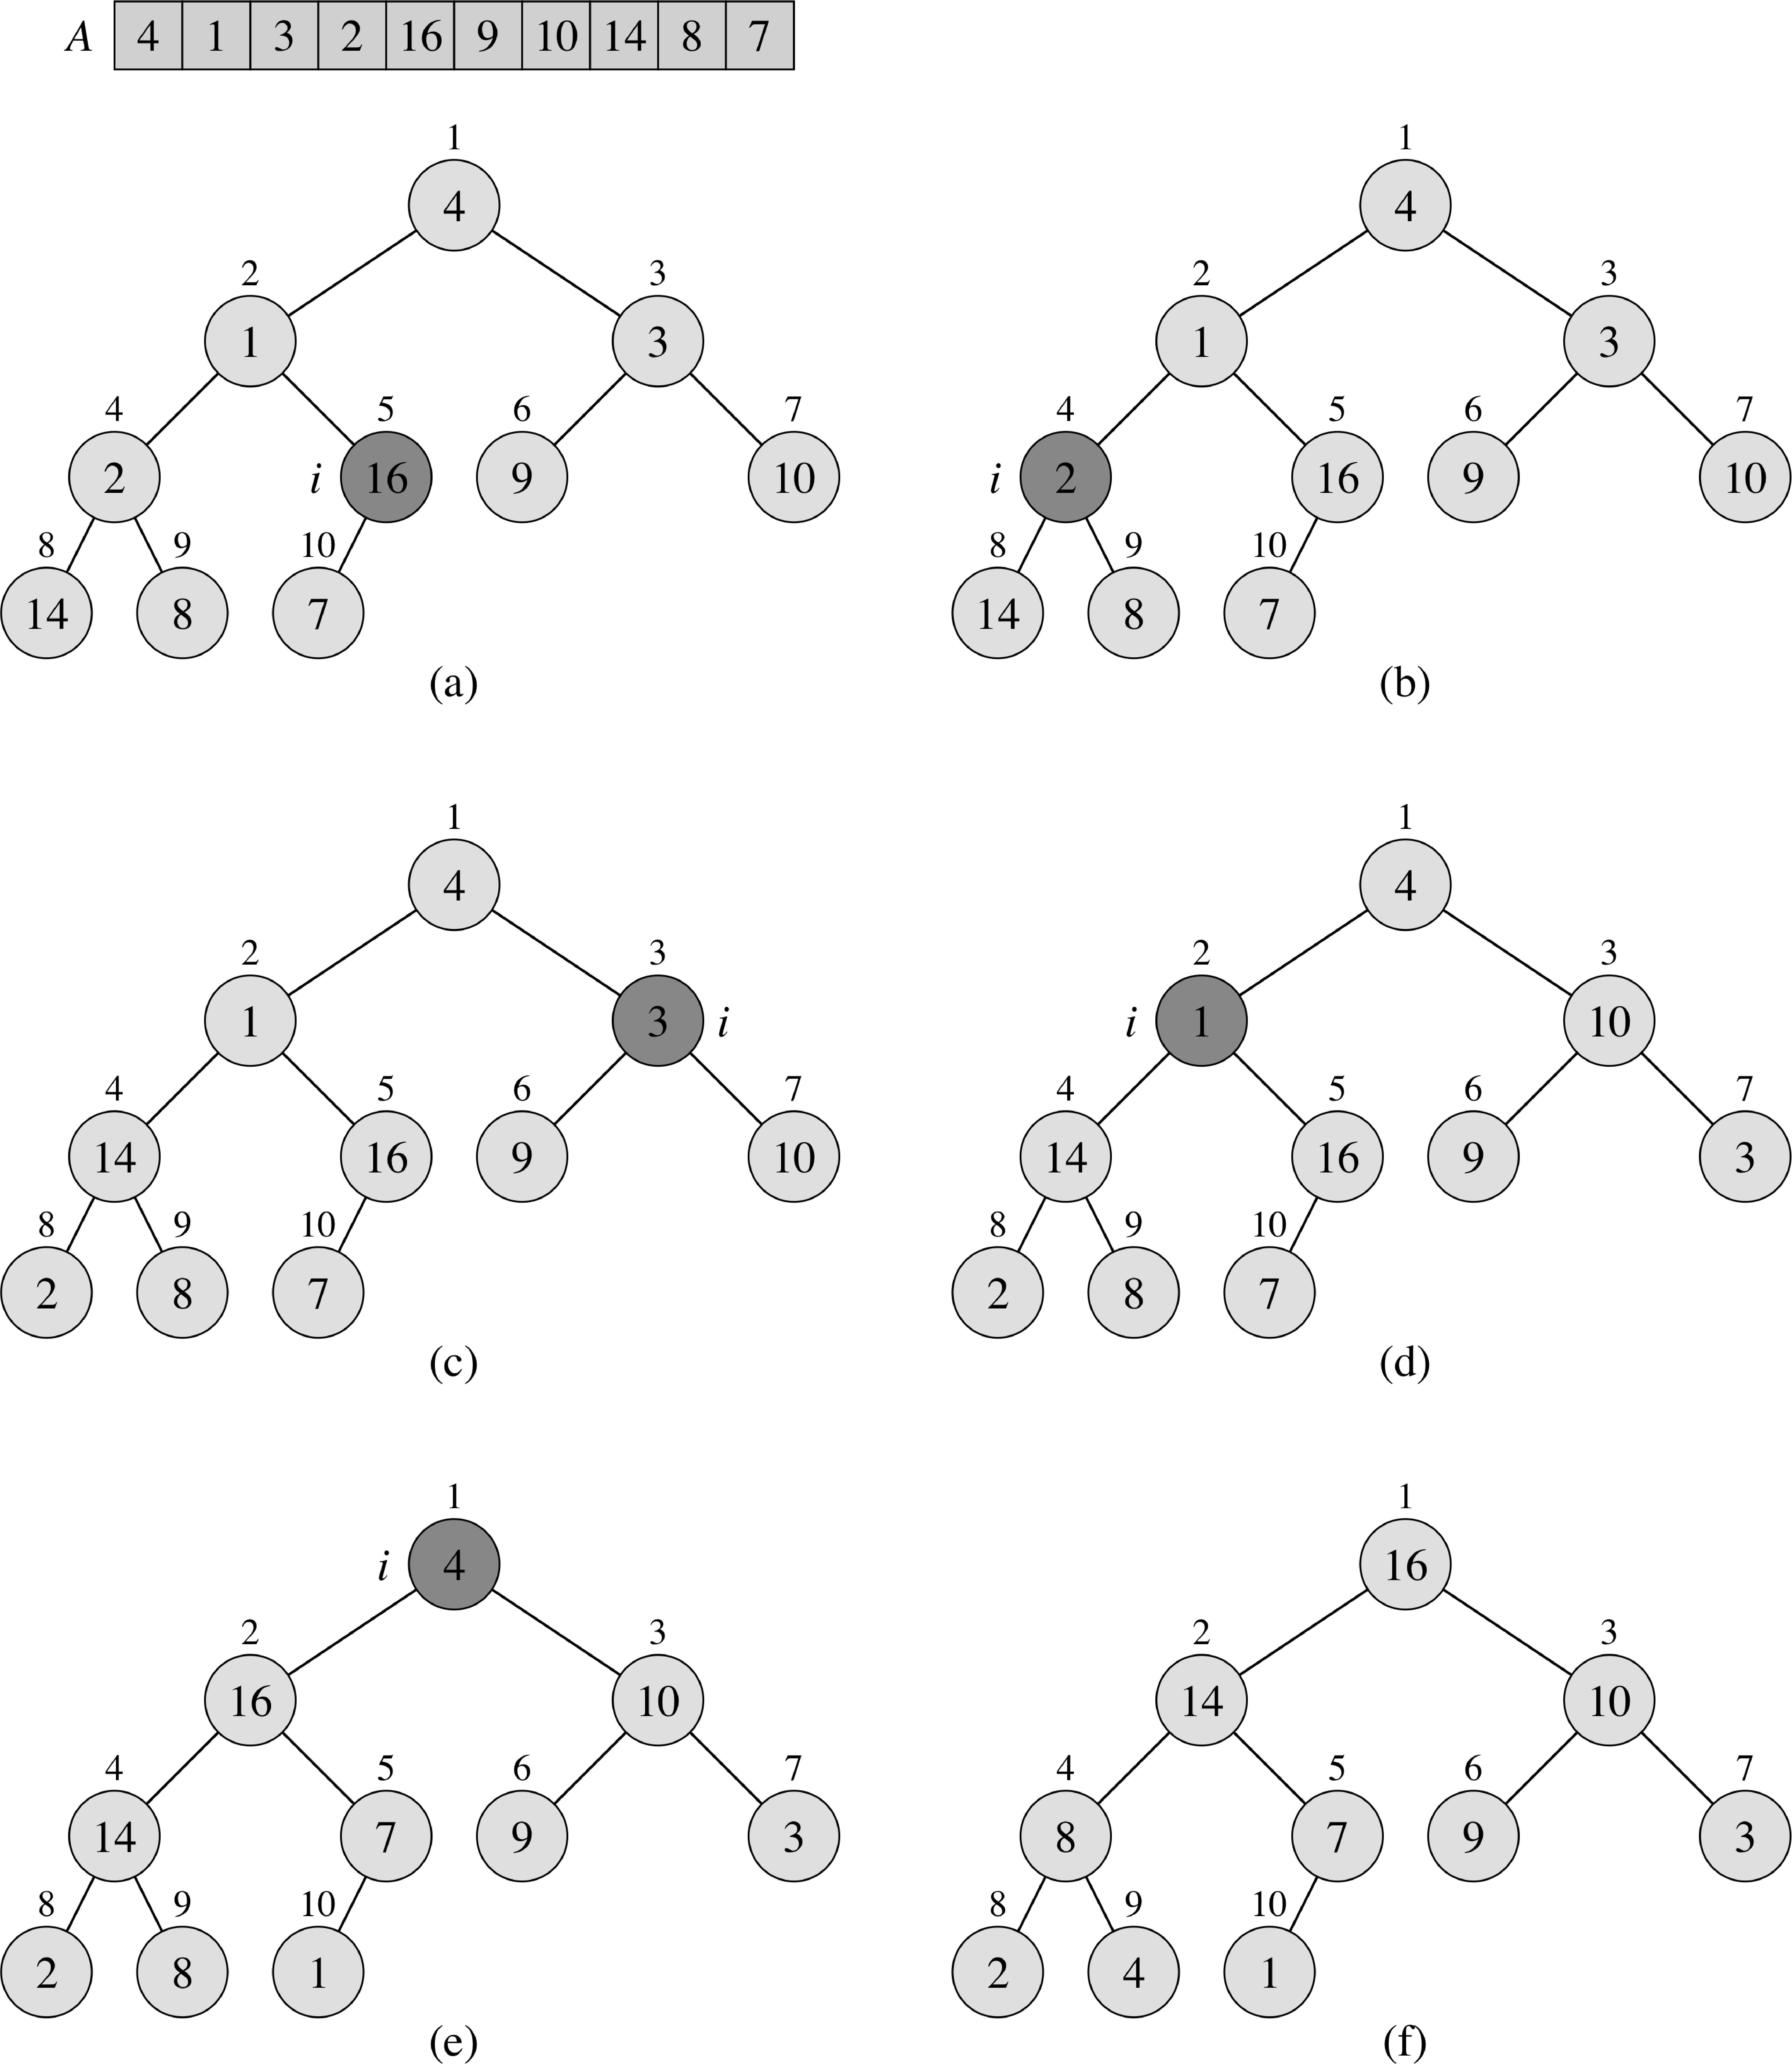
\includegraphics[height=\textheight]{Fig-6-3.pdf}

\sect{Loop invariant for {\sc Build-Max-Heap}}

\bi
\ii At start of every iteration of {\bf for} loop,
each node $i+1, i+2, \ldots, n$ is root of a max-heap.
\bi
\ii Initialization?
\ii Maintenance?
\ii Termination?
\ei
\ei
\begin{codebox}
  \Procname{$\proc{Build-Max-Heap}(A)$}
  \li \For $i=\lfloor{n/2}\rfloor \Downto 1$ \Do
  \li $\proc{Max-Heapify}(A,i,n)$
  \End
\end{codebox}

\sect{Running time of {\sc Build-Max-Heap}}
\bi
\ii Loose bound:  $O(n)$ calls to {\sc Max-Heapify}, which is $O(\lg
n)$, gives $O(n\lg n)$.
\ii We can get a tighter bound.
\bi
\ii $n$ element heap has height \flr{\lg n}
\ii $n$ element heap has at most \ceil{n/2^{h+1}} nodes of height $h$
\ii Time for {\sc Max-Heapify} on a node of height $h$ is $O(h)$
\ii Total time for  {\sc Build-Max-Heap}:
\begin{align*}
  \sum_{h=0}^{\flr{\lg n}} \ceil{\frac{n}{2^{h+1}}}O(h)
  &= O\left(n\sum_{h=0}^{\flr{\lg n}}\frac{h}{2^h}\right)
  \\
  &= O(n)
\end{align*}

\ei
\ei
Note:
\begin{align*}
  \sum_{k=0}^\infty kx^k &=\frac{x}{(1-x)^2} \tag{A.8}\\
 \sum_{k=0}^\infty k(1/2)^k &=\frac{1/2}{(1-1/2)^2} = 2
  \end{align*}


\sect{\sc Heapsort}
\bi
\ii Builds max-heap in the array.
\ii Swaps the root (the maximum) with the element at the end.
\ii Heapifies the result, with one less element.
\ii Repeat until only one element left.
\ei


\begin{codebox}
  \Procname{$\proc{Heapsort}(A)$}
  \li $\proc{Build-Max-Heap}(A)$
  \li \For $i=n$ \Downto $2$\Do
  \li exchange $A[1]$ with $A[i]$
  \li $\proc{Max-Heapify}(A,1,i-1)$
  \End
\end{codebox}


% heapsort
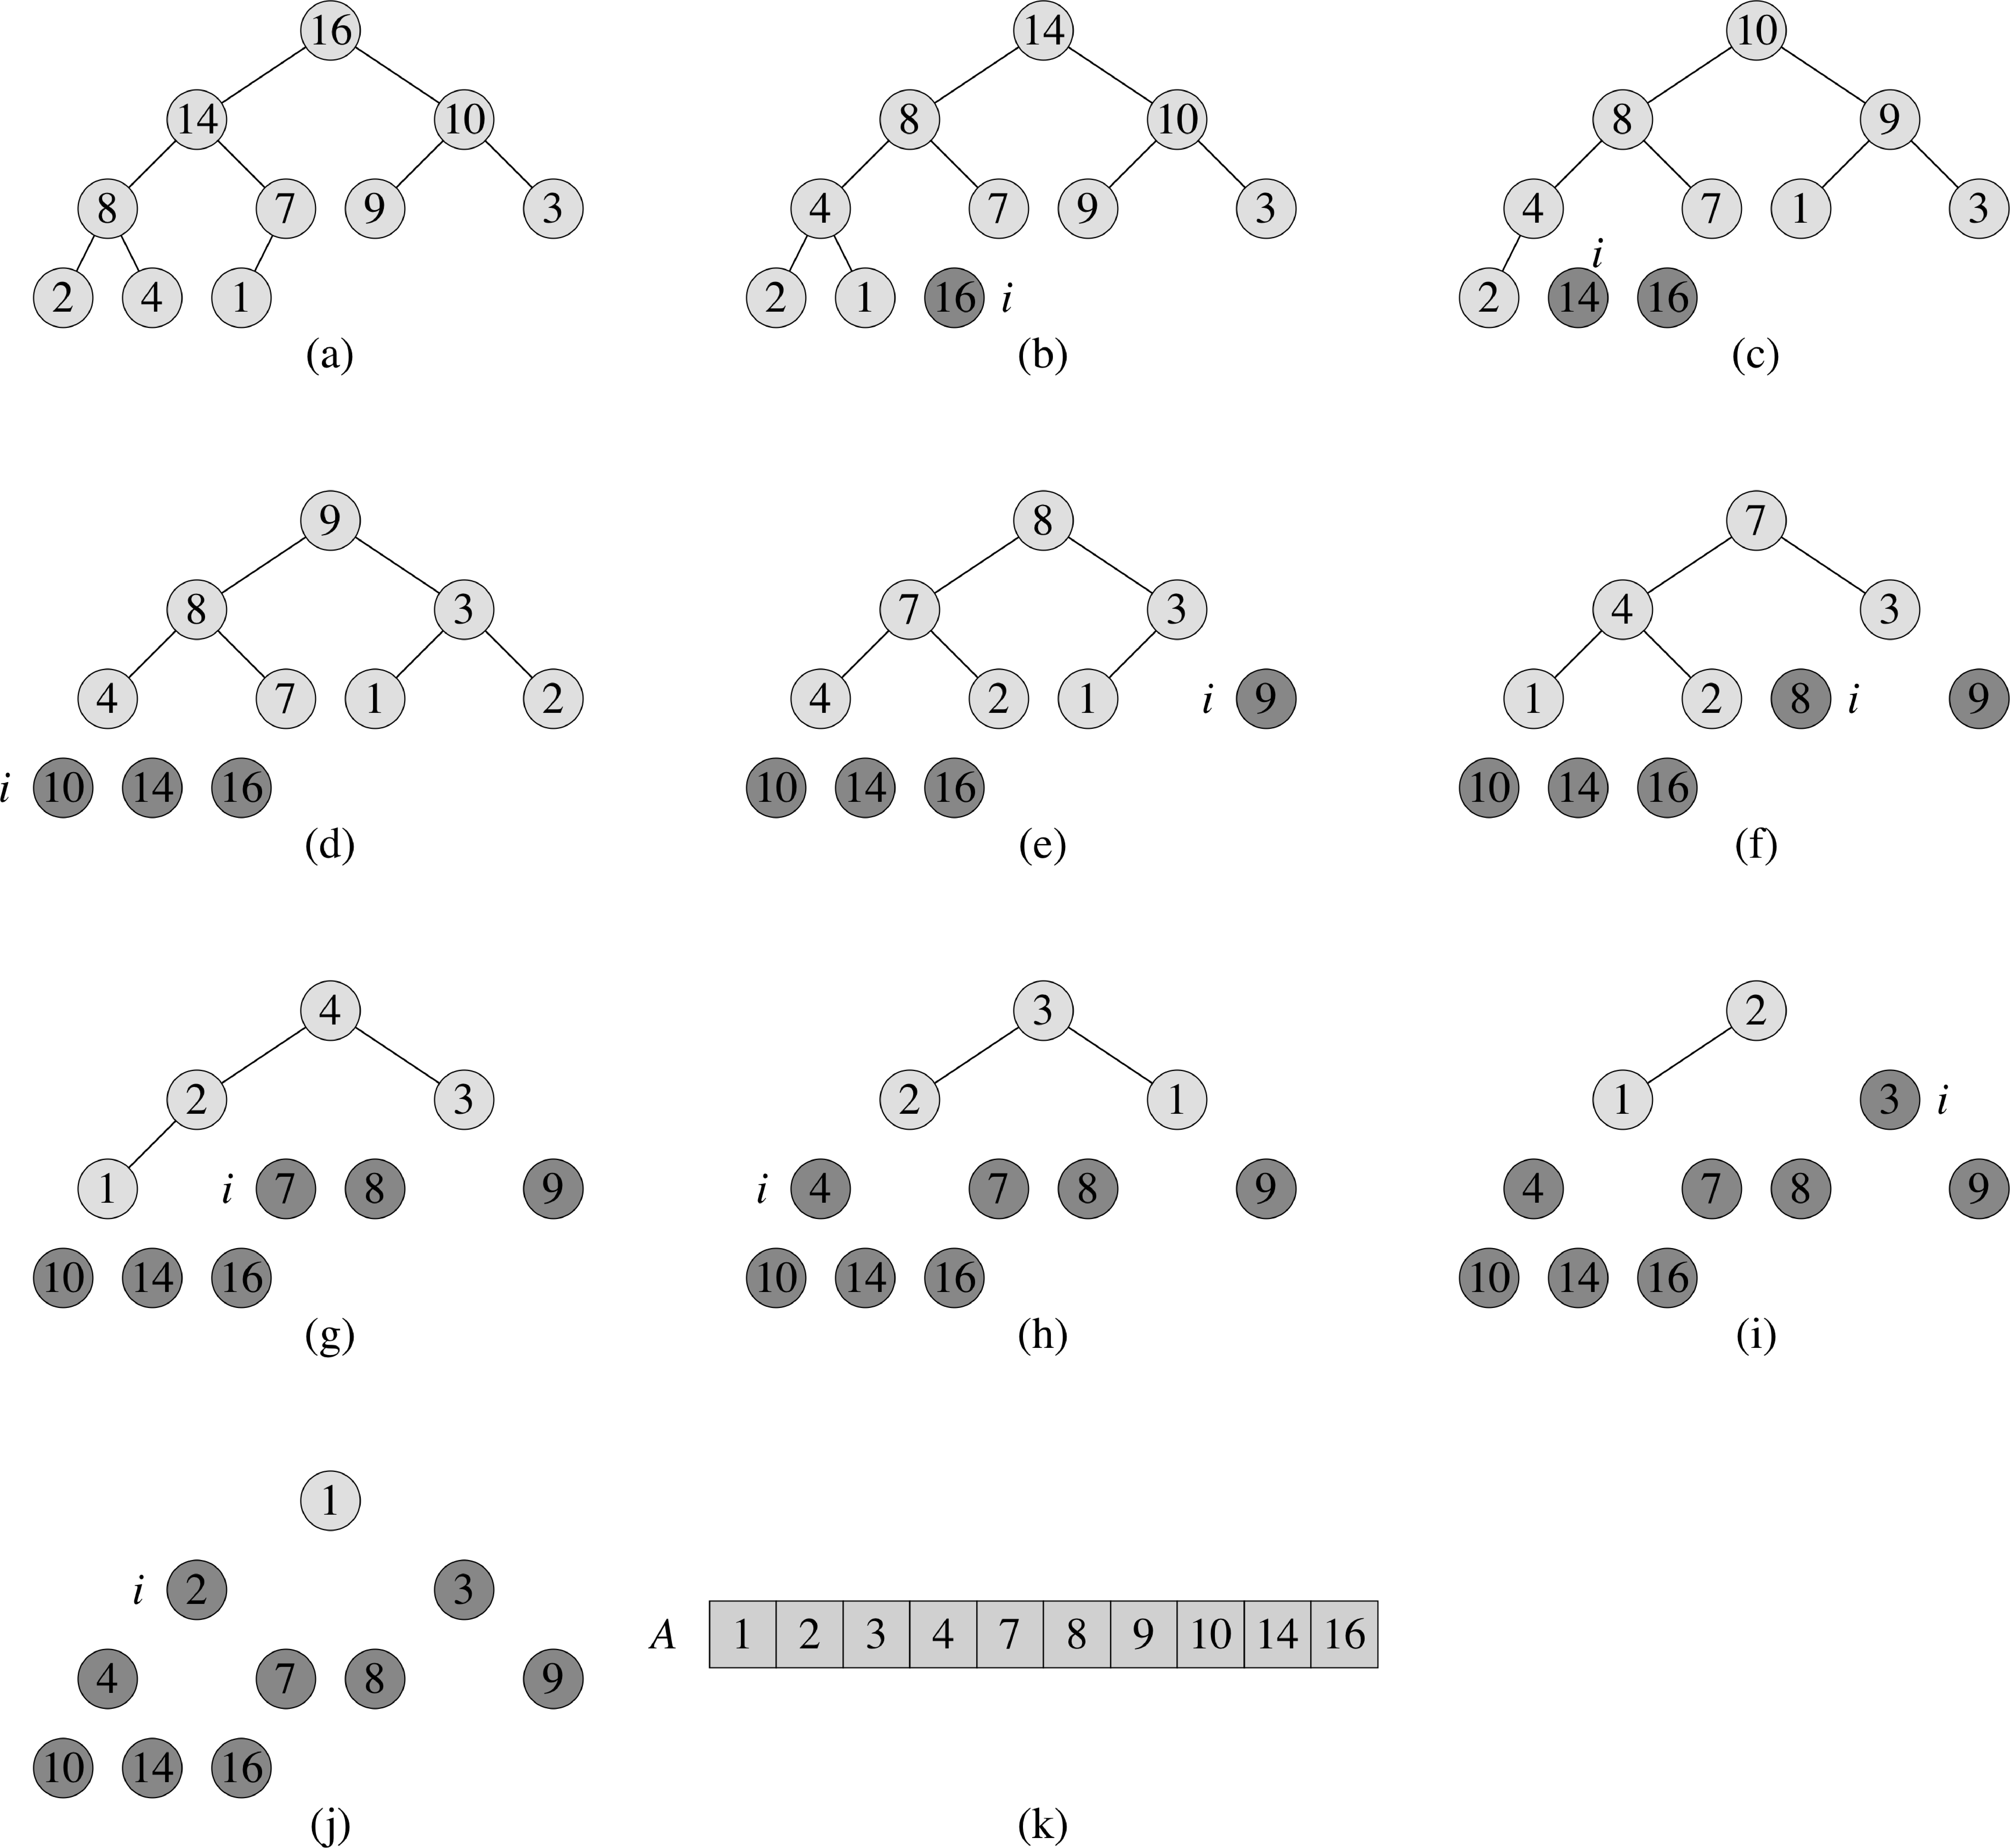
\includegraphics[height=\textheight]{Fig-6-4.pdf}


\sect{\sc Heapsort}


\begin{codebox}
  \Procname{$\proc{Heapsort}(A)$}
  \li $\proc{Build-Max-Heap}(A)$
  \li \For $i=n$ \Downto $2$\Do
  \li exchange $A[1]$ with $A[i]$
  \li $\proc{Max-Heapify}(A,1,i-1)$
  \End
\end{codebox}

\bi
\ii Analysis:  $O(n\lg n)$
\ei


\sect{Priority queue}

\bi
\ii Heaps efficiently implement priority queues.
\ii Maintains a dynamic set $S$ of elements.
\ii Each element has a {\em key}
\ii Operations:
\bi
\ii {\sc Insert$(S,x)$}
\ii {\sc Maximum$(S)$}
\ii {\sc Extract-Max$(S)$}
\ii {\sc Increase-Key$(S,x,k)$}
\ei
\ii Min priority queue similar
\ei

\sect{\sc Heap-Maximum}
\bi\ii Trivial\ii Should probably check for empty heap\ei
\begin{codebox}
  \Procname{$\proc{Heap-Maximum}(A)$}
  \li \Return $A[1]$
\end{codebox}

\bi
\ii $O(1)$
\ei

\sect{\sc Heap-Extract-Max}
\bi
\ii Make sure heap is not empty.
\ii Copy the max element (root)
\ii Make the last node the new root.
\ii Decrement the size.
\ii Re-heapify starting at the root.
\ii Return the max element copy.
\ei
\begin{codebox}
  \Procname{$\proc{Heap-Extract-Max}(A)$}
  \li \If $n < 1$ \Do
  \li \Error ``heap underflow''
\End
\li $max \gets A[1]$
\li $A[1] = A[n]$
\li $n = n-1$
\li $\proc{Max-Heapify}(A,1,n)$
\li \Return $max$
\end{codebox}

\bi
\ii $O(\lg n)$
\ei

\sect{\sc Heap-Increase-Key}
\bi
\ii Make sure $k \geq x$'s current key
\ii Update $x$'s key to $k$
\ii Traverse tree upward, swapping keys if necessary.
\ei

\begin{codebox}
  \Procname{$\proc{Heap-Increase-Key}(A,i,key)$}
  \li \If $key < A[i]$ \Do
  \li \Error ``new key is smaller than current key''
\End
\li $A[i] = key$
\li \While $i > 1$ and $A[\proc{Parent}(i)] < A[i]$ \Do
\li exchange $A[i]$ with $A[\proc{Parent}(i)]$
\li $i = \proc{Parent}(i)$
\End
\end{codebox}

\bi
\ii $O(\lg n)$
\ei

% priority queue heap increase key
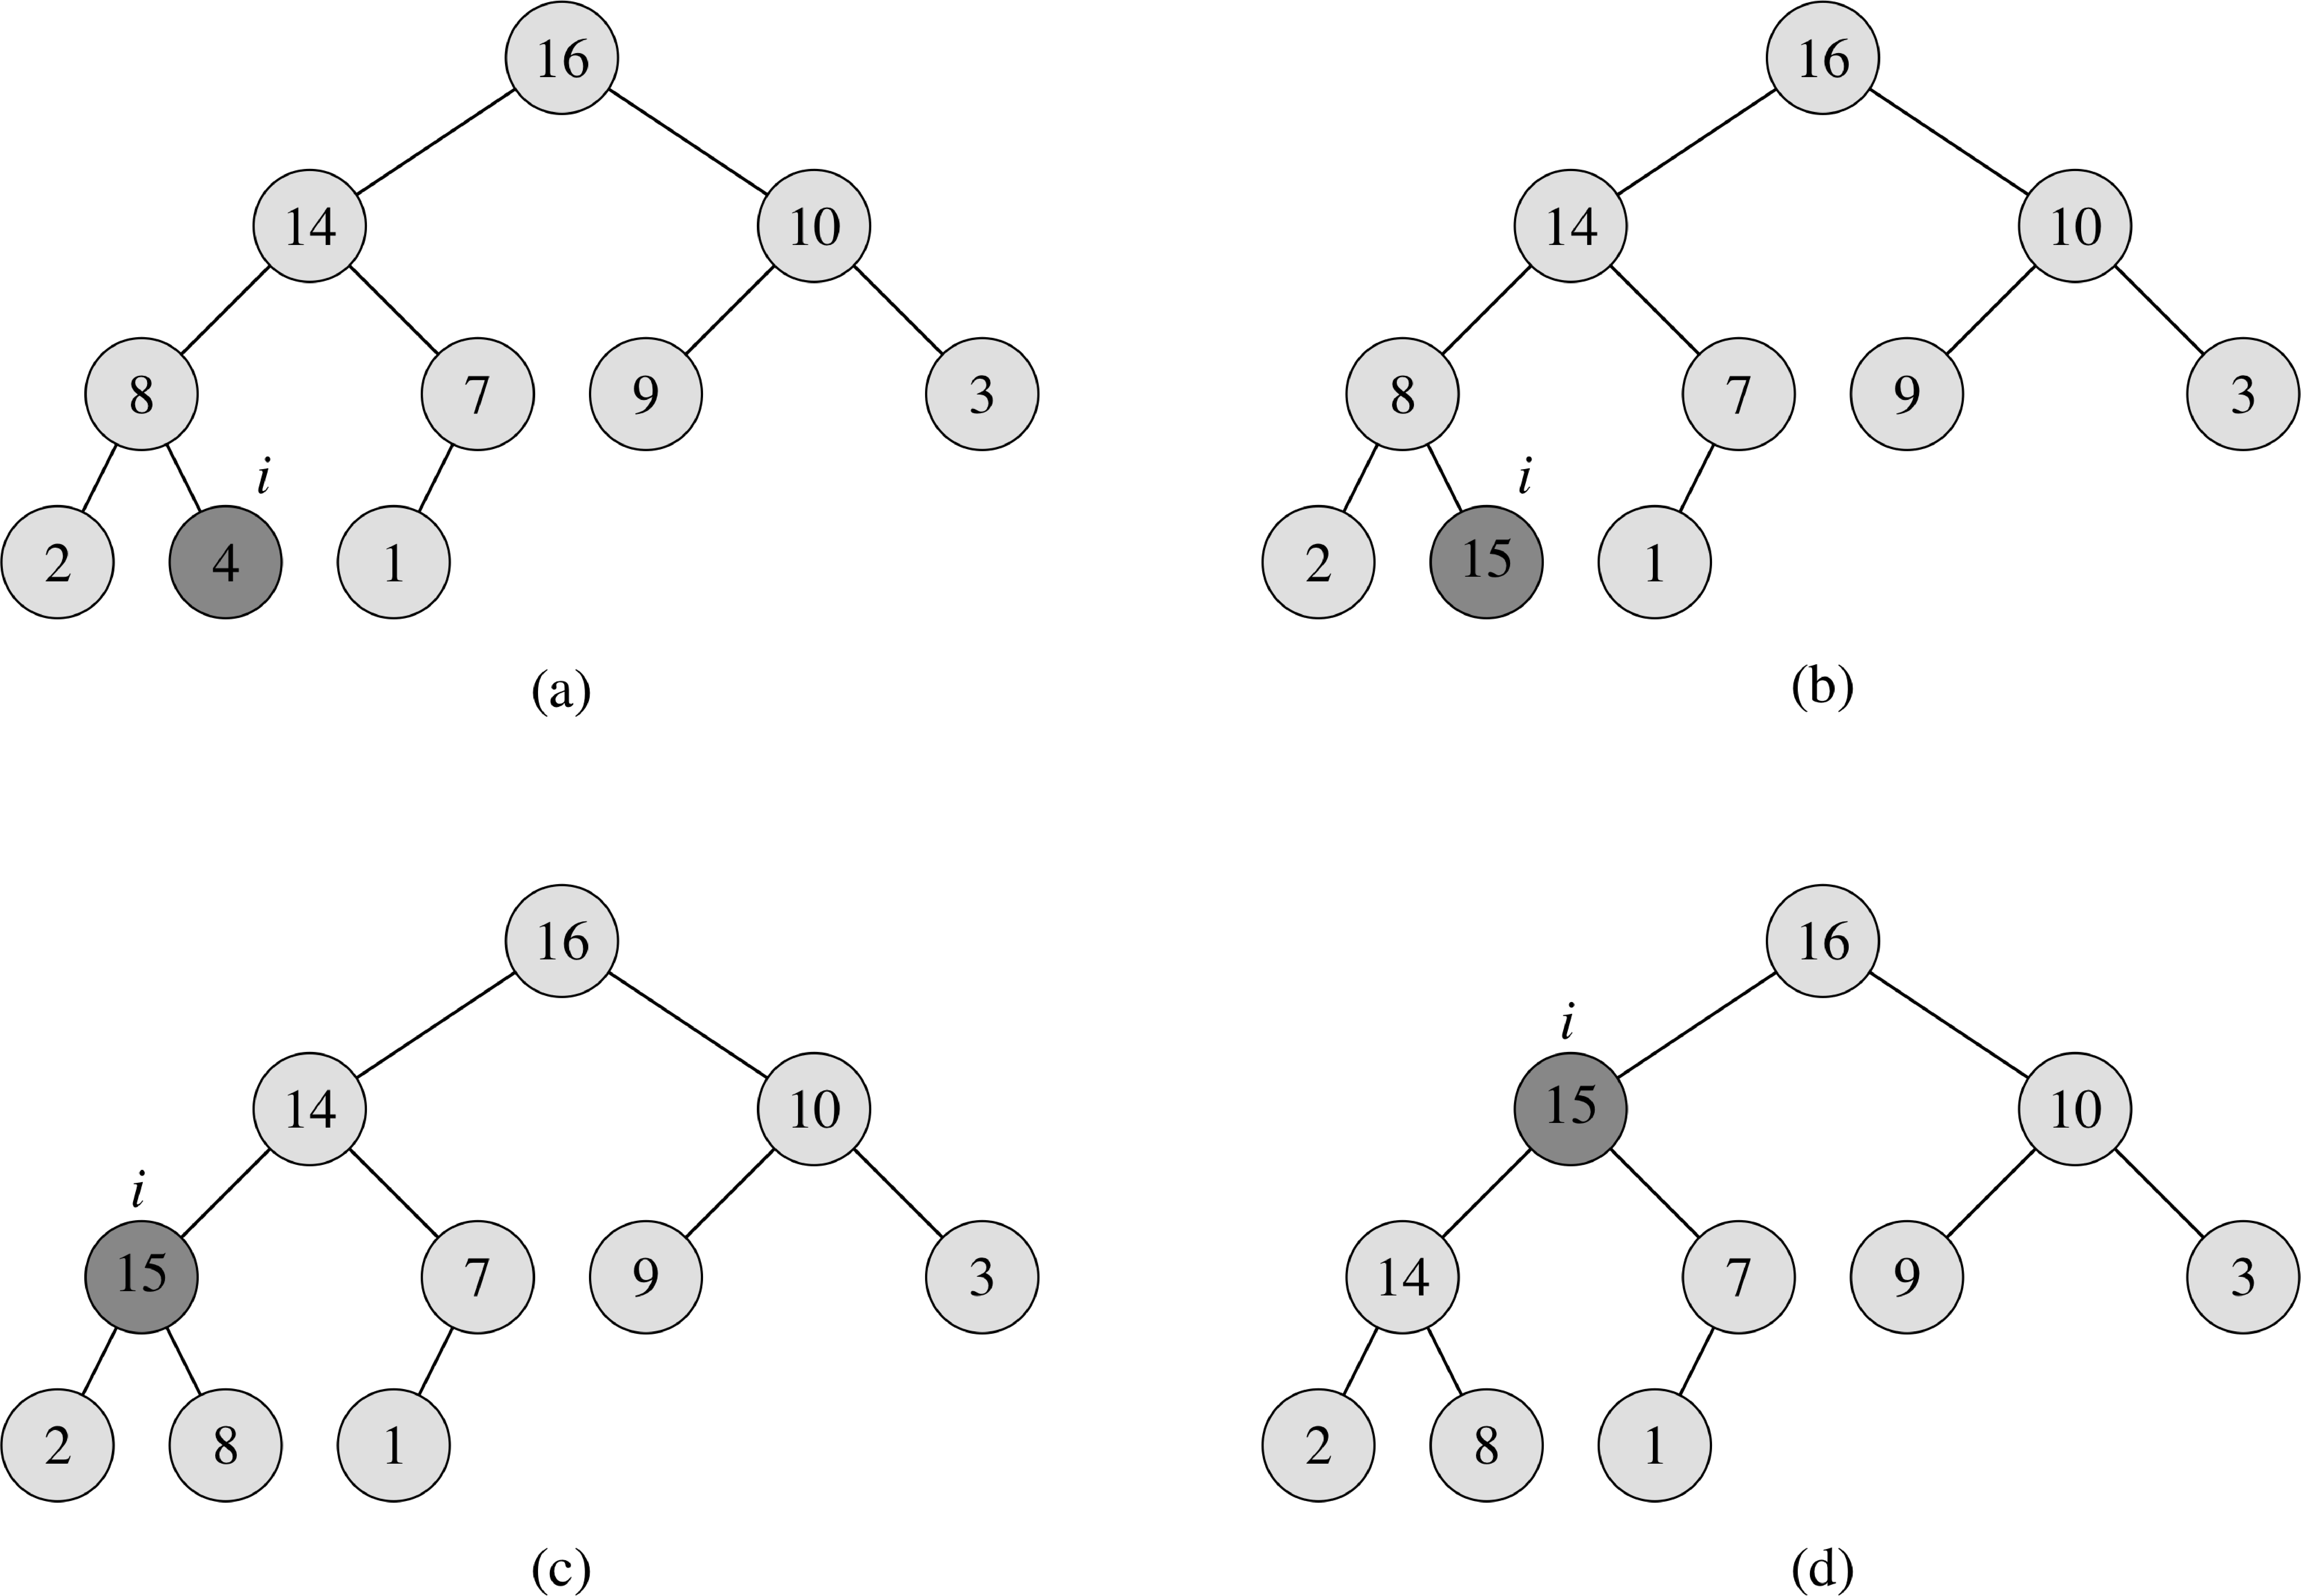
\includegraphics[height=\textheight]{Fig-6-5.pdf}

\sect{Why can't we {\tt Heap-Decrease-Key} on a max-heap?}

\sect{\sc Max-Heap-Insert}

\begin{codebox}
  \Procname{$\proc{Max-Heap-Insert}(A,key,n)$}
  \li $n \gets n+1$
  \li $A[n] \gets -\infty$
  \li $\proc{Heap-Increase-Key}(A,n,key)$
\end{codebox}

\bi
\ii $O(\lg n)$
\ei
\end{document}
